\section{Dijsktra}
\subsection{Mice and Maze}

\subsubsection*{Enunciado}
Um conjunto de ratos de laboratório está sendo treinado para escapar de um labirinto. O labirinto é composto por células, e cada célula está conectada a outras. Entretanto, há obstáculos nas passagens entre as células, o que impõe um tempo adicional para atravessá-las. Ademais, algumas passagens são unidirecionais.

Todos os ratos estão treinados e, quando colocados em uma célula arbitrária, seguem o caminho de menor tempo até a célula de saída.

No experimento, um rato é colocado em cada célula do labirinto e um temporizador é iniciado. Quando o tempo se esgota, conta-se quantos ratos conseguiram sair do labirinto.

\subsubsection*{Entrada}
A entrada inicia com um inteiro positivo indicando o número de casos de teste.

Para cada caso de teste:
\begin{itemize}
    \item A primeira linha contém um inteiro \( n \): o número total de células no labirinto.
    \item A segunda linha contém um inteiro \( E \): o número da célula de saída.
    \item A terceira linha contém um inteiro \( T \): o tempo limite do temporizador (em unidades de tempo).
    \item A quarta linha contém um inteiro \( M \): o número de conexões no labirinto.
    \item Em seguida, são fornecidos \( M \) pares de inteiros \( a \), \( b \) e um terceiro inteiro \( w \), indicando que existe uma conexão unidirecional da célula \( a \) para a célula \( b \) que leva \( w \) unidades de tempo para ser atravessada.
\end{itemize}

\subsubsection*{Saída}
Para cada caso de teste, imprima um único inteiro representando o número de ratos (um em cada célula) que conseguem alcançar a célula de saída \( E \) em no máximo \( T \) unidades de tempo.

\subsubsection*{Restrições}
\begin{itemize}
    \item \( N \le 100 \) (número de células)
    \item Cada conexão é unidirecional. O tempo para atravessar de \( a \) para \( b \) pode ser diferente do tempo de \( b \) para \( a \) (caso exista).
\end{itemize}

\subsubsection*{Exemplo}

\textbf{Entrada:}
\begin{verbatim}
1
4
2
1
8
1 2 1
1 3 1
2 1 1
2 4 1
3 1 1
3 4 1
4 2 1
4 3 1
\end{verbatim}

\textbf{Saída:}
\begin{verbatim}
3
\end{verbatim}

\subsubsection*{Solução}
\begin{lstlisting}[language=C++]
int INF = 1e9; // Defina um valor suficientemente grande

bool dijkstra(vector<vector<pair<int,int>>> graph, int start, int end, int s) {
    int n = graph.size();
    vector<int> dist(n, INF);
    dist[start] = 0;
    priority_queue<pair<int,int>, vector<pair<int,int>>, greater<pair<int,int>>> queue;
    queue.push({0, start});
    while (!queue.empty()) {
        int current_node = queue.top().second;
        queue.pop();
        for (auto edge : graph[current_node]) {
            int adj_node = edge.first;
            int weight = edge.second;
            if (dist[current_node] + weight < dist[adj_node]) {
                dist[adj_node] = dist[current_node] + weight;
                queue.push({dist[adj_node], adj_node});
            }
        }
    }
    return dist[end] <= s;
}

int main(){
    ios_base::sync_with_stdio(false);
    cin.tie(0);
    cout.tie(0);
    int cases;
    cin >> cases;
    while(cases--){
        int n, e, t;
        cin >> n;
        vector<vector<pair<int,int>>> graph(n+1);
        cin >> e >> t;
        int m;
        cin >> m;
        for (int i = 0; i < m; i++){
            int x, y, w;
            cin >> x >> y >> w;
            graph[x].push_back({y, w});
        }
        int cont = 0;
        for (int i = 1; i <= n; i++){
            if (dijkstra(graph, i, e, t)){
                cont++;
            }
        }
        cout << cont << "\n";
        if(cases > 0){
            cout << "\n";
        }
    }
}
\end{lstlisting}

\subsection{Even Obsession}

\subsubsection*{Enunciado}
Patricia é uma desenvolvedora de software brilhante, mas tem um hábito peculiar: tudo que ela faz deve ocorrer em quantidades pares. Por exemplo, ao viajar de carro, se tiver que pagar pedágio, o número de pedágios pagos deve ser par.

Em seu país, todas as estradas são de mão dupla e possuem exatamente um pedágio. Patricia está atualmente na cidade 1 e precisa visitar um cliente na cidade \(C\). Ela deseja calcular o valor mínimo total dos pedágios a pagar para ir da cidade 1 à cidade \(C\), obedecendo à sua exigência de que o número de pedágios pagos seja par.

\subsubsection*{Entrada}
Cada caso de teste consiste de:
\begin{itemize}
    \item Uma linha contendo dois inteiros \( C \) e \( V \), representando o número total de cidades e o número de estradas, respectivamente.
    \item Em seguida, \( V \) linhas, cada uma contendo três inteiros \( C_1 \), \( C_2 \) e \( G \), indicando que a estrada entre as cidades \( C_1 \) e \( C_2 \) possui um pedágio de valor \( G \).
\end{itemize}

\textbf{Observação:} As cidades são identificadas por números de 1 a \( C \). Patricia está na cidade 1 e o destino é a cidade \( C \).

\subsubsection*{Saída}
Para cada caso de teste, imprima um único inteiro: o valor mínimo total dos pedágios para ir da cidade 1 à cidade \( C \), pagando um número par de pedágios. Se não for possível, imprima \(-1\).

\subsubsection*{Restrições}
\begin{itemize}
    \item \(2 \le C \le 10^4\)
    \item \(0 \le V \le 50000\)
    \item \(1 \le C_1, C_2 \le C\)
    \item \(1 \le G \le 10^4\)
\end{itemize}

\subsubsection*{Exemplo}

\textbf{Entrada:}
\begin{verbatim}
4 4
1 2 2
2 3 1
2 4 10
3 4 6
\end{verbatim}

\textbf{Saída:}
\begin{verbatim}
12
\end{verbatim}

\subsubsection*{Solução}
\begin{lstlisting}[language=C++]
struct State {
    int cost, node, parity;
    bool operator>(const State &other) const {
        return cost > other.cost;
    }
};

void solve() {
    int C, V;
    cin >> C >> V;
    vector<vector<pair<int,int>>> graph(C+1);
    for (int i = 0; i < V; i++){
        int a, b, G;
        cin >> a >> b >> G;
        // Como as estradas são de mão dupla:
        graph[a].push_back({b, G});
        graph[b].push_back({a, G});
    }
    // Estado: (cidade, paridade dos pedágios pagos)
    vector<vector<int>> dist(C+1, vector<int>(2, 1e9));
    dist[1][0] = 0;
    priority_queue<State, vector<State>, greater<State>> pq;
    pq.push({0, 1, 0});
    while (!pq.empty()){
        State cur = pq.top();
        pq.pop();
        if (cur.cost != dist[cur.node][cur.parity])
            continue;
        for (auto edge : graph[cur.node]){
            int nxt = edge.first, w = edge.second;
            int np = (cur.parity + 1) % 2;
            if (cur.cost + w < dist[nxt][np]){
                dist[nxt][np] = cur.cost + w;
                pq.push({dist[nxt][np], nxt, np});
            }
        }
    }
    int ans = dist[C][0];
    cout << (ans == 1e9 ? -1 : ans) << "\n";
}

int main(){
    ios_base::sync_with_stdio(false);
    cin.tie(0);
    cout.tie(0);
    int t = 1;
    while(t--) solve();
    return 0;
}
\end{lstlisting}

\subsection{Trilhas Populares}

\subsubsection*{Enunciado}
Para atrair mais visitantes, o gerente de um parque nacional teve a ideia de plantar flores em ambos os lados das trilhas populares – isto é, aquelas trilhas utilizadas por pessoas comuns. Essas pessoas percorrem o parque, partindo da entrada e seguindo, pela rota de menor tempo, até o pico mais alto (onde as vistas são deslumbrantes). 

O gerente deseja saber quantos metros de flores serão necessários para cobrir ambos os lados das trilhas populares. Por exemplo, suponha que, em um determinado parque, os visitantes utilizem apenas alguns dos caminhos mais curtos da entrada ao pico; se a soma dos comprimentos desses caminhos for 1930 metros, então serão necessários \(2 \times 1930 = 3860\) metros de flores.

\subsubsection*{Entrada}
A entrada contém uma descrição do parque:
\begin{itemize}
    \item A primeira linha contém dois inteiros \(P\) e \(T\), onde \(P\) é o número de pontos de interesse (numerados de 0 a \(P-1\)), sendo o ponto 0 a entrada e o ponto \(P-1\) o pico, e \(T\) é o número de trilhas.
    \item Em seguida, são fornecidas \(T\) linhas. Cada linha contém três inteiros \(p_1\), \(p_2\) e \(l\), indicando que há uma trilha bidirecional entre os pontos \(p_1\) e \(p_2\) com comprimento \(l\) (em metros).
\end{itemize}

\subsubsection*{Saída}
Para cada caso de teste, imprima uma única linha com o total de metros de flores necessários para cobrir ambos os lados das trilhas populares.

\subsubsection*{Restrições}
\begin{itemize}
    \item \(2 \le P \le 100\).
    \item \(1 \le T \le 250\,000\).
    \item \(1 \le l \le 1\,000\).
\end{itemize}

\subsubsection*{Exemplo}

\textbf{Entrada:}
\begin{verbatim}
10 15
0 1 580
1 4 90
1 4 90
4 9 250
4 2 510
2 7 600
7 3 200
3 3 380
3 0 150
0 3 100
7 8 500
7 9 620
9 6 510
6 5 145
5 9 160
\end{verbatim}

\textbf{Saída:}
\begin{verbatim}
3860
\end{verbatim}

\subsubsection*{Solução}
\begin{lstlisting}[language=C++]
void dijkstra(vector<int> &dist, vector<vector<pair<int, int>>> &adj, int s, int n) {
    priority_queue<pair<int, int>, vector<pair<int, int>>, greater<pair<int, int>>> pq;
    dist[s] = 0;
    pq.push({0, s});

    while (!pq.empty()) {
        int d = pq.top().first;
        int u = pq.top().second;
        pq.pop();

        if (d > dist[u]) continue;

        for (auto edge : adj[u]) {
            int v = edge.first;
            int weight = edge.second;

            if (dist[v] > dist[u] + weight) {
                dist[v] = dist[u] + weight;
                pq.push({dist[v], v});
            }
        }
    }
}

void solve()
{
    int p, t;
    cin >> p >> t;
    vector<tiii> edges(t);
    vector<vii> adj(p), adj_rev(p);
    rep(i, 0, t){
        int a, b, c; cin >> a >> b >> c;
        edges[i] = {a, b, c};
        adj[a].pb({b, c});
        adj[b].pb({a, c});

        adj_rev[b].pb({a, c});
        adj_rev[a].pb({b, c});
    }
    vi dist(p, LINF), dist_rev(p, LINF);
    dijkstra(dist, adj, 0, p);
    int pico = p - 1;
    dijkstra(dist_rev, adj_rev, pico, p);
    int total = 0;
    for(auto i : edges){
        auto [a, b, c] = i;
        if(dist[a] + c + dist_rev[b] == dist[pico] ||
           dist[b] + c + dist_rev[a] == dist[pico]) total += c;
    }
    cout << 2*total << endl;
}
\end{lstlisting}

\subsection{Flip Edge}

\subsubsection*{Enunciado}
Você recebe um grafo direcionado com \(N\) vértices e \(M\) arestas. A \(i\)-ésima aresta (com \(1 \le i \le M\)) é uma aresta direcionada do vértice \(u_i\) para o vértice \(v_i\). Inicialmente, você está no vértice \(1\) e deseja chegar ao vértice \(N\). Para isso, você pode realizar as seguintes operações repetidamente:
\begin{enumerate}
    \item \textbf{Movimentar-se:} Se você estiver no vértice \(v\), escolha uma aresta direcionada que saia de \(v\) (isto é, uma aresta do tipo \(v \to u\)) e mova-se para o vértice \(u\). Essa operação custa \(1\) unidade.
    \item \textbf{Inverter arestas:} Inverta a direção de todas as arestas do grafo. Mais precisamente, se, imediatamente antes dessa operação, existia uma aresta direcionada do vértice \(v\) para o vértice \(u\), então, imediatamente após a operação, haverá uma aresta direcionada de \(u\) para \(v\). Essa operação custa \(X\) unidades.
\end{enumerate}

É garantido que, para o grafo dado, você pode alcançar o vértice \(N\) a partir do vértice \(1\) repetindo essas operações. Determine o custo total mínimo necessário para chegar ao vértice \(N\).

\subsubsection*{Restrições}
\begin{itemize}
    \item \(2 \leq N \leq 2 \times 10^5\).
    \item \(1 \leq M \leq 2 \times 10^5\).
    \item \(1 \leq X \leq 10^9\).
    \item \(1 \leq u_i, v_i \leq N\) para \(1 \le i \le M\).
    \item Todos os valores de entrada são inteiros.
\end{itemize}

\subsubsection*{Entrada}
A entrada é fornecida a partir da entrada padrão no seguinte formato:
\begin{verbatim}
N M X
u_1 v_1
u_2 v_2
.
.
.
u_M v_M
\end{verbatim}

\subsubsection*{Saída}
Imprima uma única linha contendo o custo total mínimo necessário para alcançar o vértice \(N\) a partir do vértice \(1\).

\subsubsection*{Exemplo 1}
\textbf{Entrada:}
\begin{verbatim}
5 6 5
1 2
2 4
3 1
3 5
4 3
5 2
\end{verbatim}
\textbf{Saída:}
\begin{verbatim}
4
\end{verbatim}

\subsubsection*{Exemplo 2}
\textbf{Entrada:}
\begin{verbatim}
5 6 1
1 2
2 4
3 1
3 5
4 3
5 2
\end{verbatim}
\textbf{Saída:}
\begin{verbatim}
3
\end{verbatim}

No Exemplo 1, por exemplo, o grafo se parece com a figura a seguir:

\begin{figure}
    \centering
    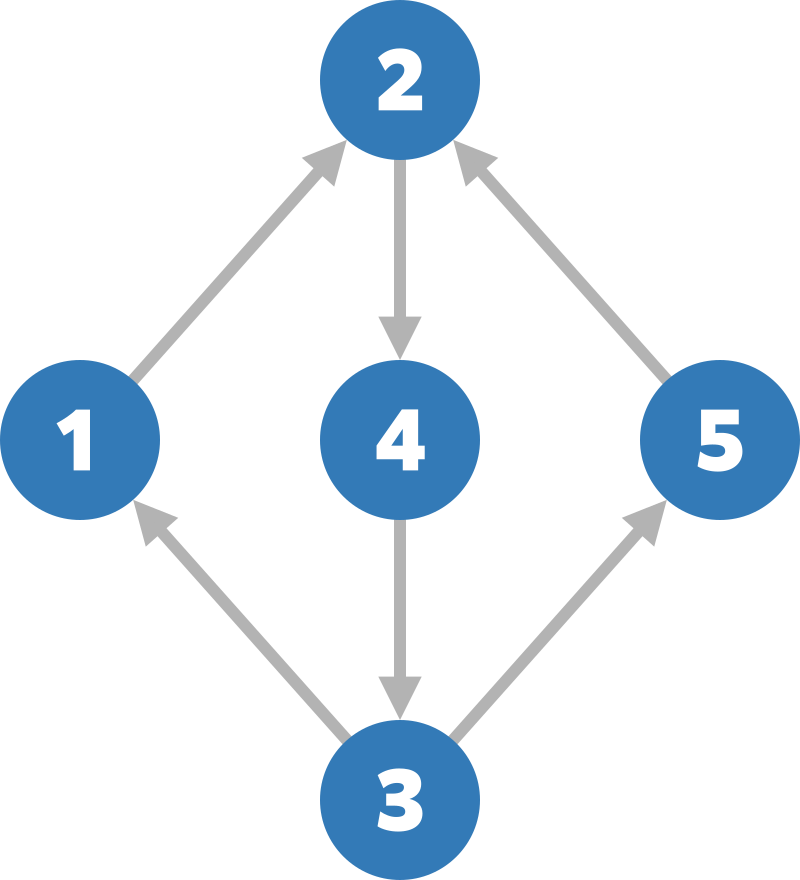
\includegraphics[width=0.5\linewidth]{flipEdge.png}
    \label{fig:enter-label}
\end{figure}

Você pode alcançar o vértice \(5\) com um custo total mínimo de \(4\) realizando, por exemplo, as seguintes operações:
\begin{itemize}
    \item Mova-se do vértice \(1\) para o vértice \(2\) (custo \(1\)).
    \item Mova-se do vértice \(2\) para o vértice \(4\) (custo \(1\)).
    \item Mova-se do vértice \(4\) para o vértice \(3\) (custo \(1\)).
    \item Mova-se do vértice \(3\) para o vértice \(5\) (custo \(1\)).
\end{itemize}

\subsubsection*{Solução}
A solução a seguir utiliza o algoritmo de Dijkstra aplicado a um estado ampliado que considera se as arestas estão no seu estado original ou invertido.

\begin{lstlisting}[language=C++]
void solve()
{
    int n, m, x; cin >> n >> m >> x;
    vvi graph(n+1), graph_inv(n+1);
    rep(i, 0, m){
        int x, y; cin >> x >> y;
        graph[x].pb(y);
        graph_inv[y].pb(x);
    }
    vvi dist(n+1, vi(2, LINF));

    priority_queue<tiii, vector<tiii>, greater<>> pq;
    dist[1][0] = 0;
    pq.push({0, 1, 0});
    while(pq.size()){
        auto [d, u, st] = pq.top(); pq.pop();
        if(dist[u][st] != d) continue;

        if(st == 0){
            for(auto v : graph[u]){
                if(dist[v][st] > d+1){
                    dist[v][st] = d+1;
                    pq.push({d+1, v, st});
                }
            }
        }else{
            for(auto v : graph_inv[u]){
                if(dist[v][st] > d+1){
                    dist[v][st] = d+1;
                    pq.push({d+1, v, st});
                }
            }
        }
        if(dist[u][1 - st] > d + x){
            dist[u][1 - st] = d + x;
            pq.push({dist[u][1-st], u, 1 - st});
        }
    }
    cout << min(dist[n][0], dist[n][1]) << endl;
}
\end{lstlisting}

\subsection{Audiophobia}

\subsubsection*{Enunciado}
Considere-se sortudo! Considere-se sortudo por ainda estar respirando e se divertindo participando deste concurso. Mas tememos que muitos de seus descendentes possam não ter esse privilégio. Pois, como você sabe, somos moradores de uma das cidades mais poluídas do mundo. A poluição está em toda parte, tanto no ambiente quanto na sociedade, e nossa falta de consciência só agrava a situação.

Por ora, porém, vamos considerar apenas um tipo de poluição – a poluição sonora. O nível de intensidade do som é geralmente medido em decibéis e sons com intensidade de 130 decibéis ou mais são considerados dolorosos. O nível de uma conversa normal é de 60 a 65 decibéis, enquanto o do tráfego intenso é de 70 a 80 decibéis.

Considere o seguinte mapa da cidade, onde as arestas representam ruas e os nós representam cruzamentos. O número inteiro em cada aresta indica o nível médio de intensidade sonora (em decibéis) na rua correspondente. Por exemplo, para ir do cruzamento A ao cruzamento G, você pode seguir o caminho A-C-F-G, o que exige tolerar um som de até 140 decibéis. Já para os caminhos A-B-E-G, A-B-D-G e A-C-F-D-G, é necessário tolerar, respectivamente, 90, 120 e 80 decibéis. Observa-se que o caminho A-C-F-D-G é o mais confortável, pois não demanda tolerância a mais de 80 decibéis.

Neste problema, dada a descrição do mapa da cidade, você deve determinar o nível mínimo de intensidade sonora (em decibéis) que você precisa tolerar para ir de um cruzamento a outro.

\subsubsection*{Entrada}
A entrada pode conter vários casos de teste. A primeira linha de cada caso de teste contém três inteiros \(C\), \(S\) e \(Q\), separados por espaços, onde:
\begin{itemize}
    \item \(C\) indica o número de cruzamentos (os cruzamentos são numerados de 1 a \(C\));
    \item \(S\) representa o número de ruas;
    \item \(Q\) é o número de consultas.
\end{itemize}
Cada uma das próximas \(S\) linhas contém três inteiros \(c_1\), \(c_2\) e \(d\), indicando que o nível médio de intensidade sonora na rua que conecta os cruzamentos \(c_1\) e \(c_2\) (com \(c_1 \neq c_2\)) é \(d\) decibéis.
Cada uma das próximas \(Q\) linhas contém dois inteiros \(c_1\) e \(c_2\) (\(c_1 \neq c_2\)), representando uma consulta: qual é o nível mínimo de intensidade sonora que você precisa tolerar para ir do cruzamento \(c_1\) para o cruzamento \(c_2\)?
A entrada termina com uma linha contendo três zeros separados por espaços.

\subsubsection*{Saída}
Para cada caso de teste, seu programa deve imprimir:
\begin{itemize}
    \item Primeiramente, o número do caso de teste (começando em 1) no formato “Case \#\(i\)”;
    \item Em seguida, para cada consulta, imprima uma linha contendo um inteiro, que é o nível mínimo de intensidade sonora (em decibéis) que deve ser tolerado para ir do primeiro ao segundo cruzamento da consulta. Se não existir um caminho entre eles, imprima “no path”.
\end{itemize}
Imprima uma linha em branco entre dois casos de teste consecutivos.

\subsubsection*{Exemplo de Entrada}
\begin{verbatim}
7 9 3
1 2 50
1 3 60
2 4 120
2 5 90
3 6 50
4 6 80
4 7 70
5 7 40
6 7 140
1 7
2 6
6 2
7 6 3
1 2 50
1 3 60
2 4 120
3 6 50
4 6 80
5 7 40
7 5
1 7
2 4
0 0 0
\end{verbatim}

\subsubsection*{Exemplo de Saída}
\begin{verbatim}
Case #1
80
60
60

Case #2
40
no path
80
\end{verbatim}



\begin{lstlisting}
int main()
{
    ios::sync_with_stdio(0);
    cin.tie(0);
    cout.tie(0);
    int n, m, q;
    int c = 0;
    while (cin >> n >> m >> q && (n || m || q))
    {
        vector<vector<int>> dist(n + 1, vector<int>(n + 1, INF));
        for (int i = 1; i <= n; i++)
        {
            dist[i][i] = 0;
        }

        for (int i = 0; i < m; i++)
        {
            int a, b, c;
            cin >> a >> b >> c;
            dist[a][b] = dist[b][a] = c;
        }

        for (int k = 1; k <= n; k++)
        {
            for (int i = 1; i <= n; i++)
            {
                for (int j = 1; j <= n; j++)
                {

                    dist[i][j] = min(dist[i][j], max(dist[i][k], dist[k][j]));
                }
            }
        }
        if(c) cout << endl ;
        cout << "Case #" << ++c << endl;
        while (q--)
        {
            int x, y;
            cin >> x >> y;
            ((dist[x][y] == INF) ? cout << "no path" : cout << dist[x][y]);

            cout << endl;
        }
    }
}
\end{lstlisting}